\documentclass[11pt]{article}

\usepackage{a4wide}
\usepackage[utf8]{inputenc}
\usepackage[russian]{babel}
\usepackage{graphicx}
\usepackage{indentfirst} 
\usepackage{amsmath}
\usepackage{amssymb}
\usepackage{amsthm}


\begin{document}

\thispagestyle{empty}

\begin{center}
\ \vspace{-3cm}


\includegraphics[width=0.5\textwidth]{msu.eps}\\
{\scshape Московский государственный университет имени М.~В.~Ломоносова}\\
Факультет вычислительной математики и кибернетики\\
Кафедра системного анализа

\vfill

{\LARGE Отчёт по самому важному предмету}

\vspace{1cm}

{\Huge\bfseries <<Практикум на Matlab>>}
\end{center}

\vspace{1cm}

\begin{flushright}
  \large
  \textit{Студент 315 группы}\\
  Д.\,М.~Сотников

  \vspace{5mm}

  \textit{Руководитель практикума}\\
  к.ф.-м.н., доцент П.\,А.~Точилин
\end{flushright}

\vfill

\begin{center}
Москва, 2019
\end{center}

\newpage
\section{Постановка задачи}
Рассматривается краевая задача для уравнения Лапласа
\begin{equation}
\left\{
	\begin{aligned}
		& u_{xx}''\left(x, \, y\right) + u_{yy}''\left(x, \, y\right) - \mu u\left(x\, y\right) = \label{problem}
		f\left(x, \, y\right), \quad \left(x, \, y\right) \in \left[0, \, 1\right] \times \left[0, \, 1\right], \\
		& u\left(x, \, 0\right) \equiv u\left(x, \, 1\right) \equiv \xi\left(x\right), \\
		& u\left(0, \, y\right) \equiv u\left(1, \, y\right) \equiv \eta\left(y\right), \\ 
		& \xi\left(0\right) = \xi\left(1\right) = \eta\left(0\right) = \eta\left(1\right).
	\end{aligned}	
\right.
\end{equation}

Здесь функция $f\left(\cdot\, , \, \cdot\right)$ непрерывно дифференцируема в $\left[0, \, 1\right]
\times \left[0, \, 1\right]$, функции $\xi\left(\cdot\right), \eta\left(\cdot\right)$ 
непрерывно дифференцируемы на отрезке $\left[0, \, 1\right]$, а вещественный параметр $\mu > 0$.

Для данной задачи нужно построить алгоритм поиска численного решения, основанный
на быстром преобразовании Фурье, а именно необходимо реализовать функцию 
solveDirichlet(fHandle, xiHandle, etaHandle, mu, N, M), возвращающую значение решения на сетке размера N на M.
Первые три аргумента функции представляют собой указатели на функции $f\left(\cdot\, , \, \cdot\right), \ \xi\left(\cdot\right), \ \eta\left(\cdot\right)$ соответственно. Затем
передается значение параметра $\mu$ и размер сетки.

\newpage
\section{Алгоритм решения}
Для решения поставленной задачи используется разностная схема, в которой уравнение 
Лапласа принимает вид
\begin{equation} 
\begin{split}
&\dfrac{y_{k+1,l}-2y_{k,l}+y_{k-1,l}}{h_x^2} + 
\dfrac{y_{k,l+1}-2y_{k,l}+y_{k,l-1}}{h_y^2} - \mu y_{k,l} = \phi_{k,l}, \\ \label{approx}
&y_{k,0} = y_{k,M} = \xi_k, \quad y_{0,l} = y_{N,l} = \eta_l, \quad k = 1,\ldots,N-1, \quad l = 1,\ldots,M-1.
\end{split}
\end{equation}

Здесь на сетке $x_k = \frac{k}{N},\ y_l = \frac{l}{M},\ h_x=\frac{1}{N}, \ h_y=\frac{1}{M}$ задаются функции \\
$y_{k,l} = u\left(x_k, \, y_l\right),\ \phi_{k,l} = f\left(x_k, \, y_l\right), \
\xi_k = \xi\left(x_k\right),\ \eta_l = \eta\left(y_l\right).$

Пусть $\left\{a_{s,p}\right\}, \ \left\{b_{s,p}\right\}, \ s = 1,\ldots,N-1, \ p = 1,\ldots,M-1$ задают обратное двумерное преобразование для $y_{k,m}$ и $\phi_{k,m}$ соответствено. Тогда 
$$ y_{k,m}=\sum_{s=0}^{N-1}\sum_{p=0}^{M-1}a_{s,p}e^{-2\pi i \left(\frac{ks}{N} + \frac{mp}{M}\right)}$$
$$ \phi_{k,m}=\sum_{s=0}^{N-1}\sum_{p=0}^{M-1}b_{s,p}e^{-2\pi i \left(\frac{ks}{N} + \frac{mp}{M}\right)}$$

Подставляя эти соотношения в разностную схему (\ref{approx}) и приравнивая коэффициенты при экспонентах, получаем
\begin{equation}
a_{s,p}c_{s,p}= b_{s,p}, \label{ac=b}
\end{equation}
где $$c_{s,p} = -4N^2\sin^2\left(\frac{\pi s}{N}\right)-4M^2\sin^2\left(\frac{\pi p}{M}\right) - \mu.$$

Для удовлетворения граничным условиям необходимо специальным образом подобрать значения $\phi_{k,0}, \, \phi_{0,l}$. Для этого представим
$b_{s,p}$ в виде 
\begin{multline} 
b_{s,p}=\dfrac{1}{MN}\sum_{k=0}^{N-1}\sum_{m=0}^{M-1}\phi_{k,m}e^{2\pi i \left(\frac{ks}{N} + \frac{mp}{M}\right)}= \\
\dfrac{1}{MN}\sum_{l=0}^{M-1}\phi_{0,l}e^{2\pi i \left(\frac{lp}{M}\right)} + 
\dfrac{1}{MN}\sum_{l=0}^{M-1}\phi_{l,0}e^{2\pi i \left(\frac{ls}{N}\right)} - \dfrac{1}{MN}\phi_{0,0} + \overline{b_{s,p}}.\label{b}
\end{multline}
Здесь $\overline{b_{s,p}} = \dfrac{1}{MN}\sum\limits_{k=1}^{N-1}\sum\limits_{m=1}^{M-1}\phi_{k,m}e^{2\pi i \left(\frac{ks}{N} + \frac{mp}{M}\right)}$.
Заметим, что $\overline{b_{s,p}}$ можно вычислить, применив обратное двумерное преобразование преобразование Фурье (функция ifft2 в Matlab) к матрице 
\[ 
\begin{pmatrix}
	0 & 0 & \dots & 0 \\
	0 & \phi_{1,1} & \dots & \phi_{1,M-1} \\
	\hdotsfor{4} \\
	0 & \phi_{N-1,1} & \dots & \phi_{N-1, M-1}
\end{pmatrix}
\]

\newpage
Поскольку
$$ \eta_m = y_{0,m} = \sum_{s=0}^{N-1}\sum_{p=0}^{M-1}a_{s,p}e^{-2\pi i \left(\frac{mp}{M}\right)} = 
\sum_{s=0}^{N-1}\sum_{p=0}^{M-1}\dfrac{b_{s,p}}{c_{s,p}}e^{-2\pi i \left(\frac{mp}{M}\right)},$$
$$ \xi_k = y_{k,0} = \sum_{s=0}^{N-1}\sum_{p=0}^{M-1}a_{s,p}e^{-2\pi i \left(\frac{ks}{N}\right)} = 
\sum_{s=0}^{N-1}\sum_{p=0}^{M-1}\dfrac{b_{s,p}}{c_{s,p}}e^{-2\pi i \left(\frac{ks}{N}\right)},$$
подставляя (\ref{b}) в эти выражения, получим систему линейных алгебраических уравнений относительно
$\phi_{0,0}, \ldots, \phi_{0,M-1}, \phi_{1,0}, \ldots, \phi_{N-1,0}$:
\begin{multline}
\eta_m = \dfrac{1}{MN}\sum_{l=0}^{M-1}\phi_{0,l}\sum_{s=0}^{N-1}\sum_{p=0}^{M-1}\dfrac{1}{c_{s,p}}e^{-2\pi i\frac{mp}{M}}e^{2\pi i\frac{lp}{M}} \\
+ \dfrac{1}{MN}\sum_{l=1}^{N-1}\phi_{l,0}\sum_{s=0}^{N-1}\sum_{p=0}^{M-1}\dfrac{1}{c_{s,p}}e^{-2\pi i\frac{mp}{M}}e^{2\pi i\frac{ls}{N}}
- \sum_{s=0}^{N-1}\sum_{p=0}^{M-1}\dfrac{\overline{b_{s,p}}}{c_{s,p}}e^{-2\pi i\frac{mp}{M}}, \quad m = 0,\ldots,M-1
\end{multline}
\begin{multline}
\xi_k = \dfrac{1}{MN}\sum_{l=0}^{M-1}\phi_{0,l}\sum_{s=0}^{N-1}\sum_{p=0}^{M-1}\dfrac{1}{c_{s,p}}e^{-2\pi i\frac{ks}{N}}e^{2\pi i\frac{lp}{M}} \\
+ \dfrac{1}{MN}\sum_{l=1}^{N-1}\phi_{l,0}\sum_{s=0}^{N-1}\sum_{p=0}^{M-1}\dfrac{1}{c_{s,p}}e^{-2\pi i\frac{ks}{N}}e^{2\pi i\frac{ls}{N}}
- \sum_{s=0}^{N-1}\sum_{p=0}^{M-1}\dfrac{\overline{b_{s,p}}}{c_{s,p}}e^{-2\pi i\frac{ks}{N}}, \quad k = 1,\ldots,N-1
\end{multline}

Уравнение на $\xi_0$ не было включено в систему, так как $\xi_0 = \eta_0$ по постановке задачи.

Для вычисления коэффициентов вида 
$\dfrac{1}{MN}\sum\limits_{s=0}^{N-1}\sum\limits_{p=0}^{M-1}\dfrac{1}{c_{s,p}}e^{-2\pi i\frac{mp}{M}}e^{2\pi i\frac{lp}{M}}$ достаточно
просуммировать матрицу $\left\{\frac{1}{c_{s,p}}\right\}$ по $s$, применить обратное преобразование по $p$ с помощью функции fft и 
сделать циклический сдвиг на $m$ вправо.

Коэффициенты вида 
$\dfrac{1}{MN}\sum\limits_{s=0}^{N-1}\sum\limits_{p=0}^{M-1}\dfrac{1}{c_{s,p}}e^{-2\pi i\frac{mp}{M}}e^{2\pi i\frac{ls}{N}}$ 
вычисляются последовательным применением прямого преобразования Фурье к строкам матрицы  $\left\{\frac{1}{c_{s,p}}\right\}$, а затем
обратного преобразования (ifft) к её столбцам.

Правая часть системы вычиляется так же с помощью прямого преобразования fft.

Решив систему, построим матрицу $\left\{\phi_{k,m}\right\},\ k = 1,\ldots,N-1, \ m = 1,\ldots,M-1$.
Применяя к ней двумерное обратное преобразование Фурье (ifft2), находим матрицу
 $\left\{b_{s,p}\right\},\ s = 1,\ldots,N-1, \ p = 1,\ldots,M-1$.
С помощью формулы (\ref{ac=b}) вычислим значения $\left\{a_{s,p}\right\},\ s = 1,\ldots,N-1, \ p = 1,\ldots,M-1$ и применим к ним
прямое преобразование Фурье fft2, найдя тем самым искомое решение 
$\left\{y_{k,m}\right\},\ k = 1,\ldots,N-1, \ m = 1,\ldots,M-1$.

\newpage
\section{Вычисление аналитического решения}
В этом разделе будет вычислено аналитическое решение задачи (\ref{problem}) для функции 
$f\left(x, \, y\right) = e^{2x}\cos\left(3x\right)-y^2e^y = f_1(x) + f_2(y).$ Исходя из вида $f$ решение ищется в виде 
$$u(x, \, y) = u_1(x) + u_2(y), \quad u_1(0) = u_1(1) = u_1^0, \quad u_2(0) = u_2(1) = u_2^0,$$
числа $u_1^0$ и $u_2^0$ известны.

При этих условиях задача (\ref{problem}) распадается на две одномерные краевые задачи
\begin{equation}
\left\{
	\begin{aligned}
	& u_1''-\mu u_1 = e^{2x}\cos(3x) \label{bvp1} \\
	& u_1(0) = u_1(1) = u_1^0 
	\end{aligned}	
\right.
\end{equation}

\begin{equation}
\left\{
	\begin{aligned}
	& u_2''-\mu u_2 = -y^2 e^y \label{bvp2} \\
	& u_2(0) = u_2(1) = u_2^0 
	\end{aligned}	
\right.
\end{equation}

Общее решение однородного уравнения для обеих задач имеет вид
$$u(x) = c_1 e^{\sqrt{\mu}x} + c_2 e^{-\sqrt{\mu}x}.$$

Для первой краевой задачи методом вариации постоянных находим
$$c_1'(x) = \frac{1}{2\sqrt{\mu}}e^{x\left(2-\sqrt{\mu}\right)}\cos(3x), \qquad
c_2'(x) = -\frac{1}{2\sqrt{\mu}}e^{x\left(2+\sqrt{\mu}\right)}\cos(3x).$$

Интегрируя эти выражения получим 
$$c_1 = \frac{\left(3\sin\left(3x\right)+\left(2-\sqrt{\mu}\right)\cos\left(3x\right)\right)e^{x\left(2-\sqrt{\mu}\right)}}{2\sqrt{\mu}
\left(\mu-4\sqrt{\mu}+13\right)} + d_1 = c_1(x) + d_1, \quad d_1 \in \mathbb{R}$$
$$c_2 = -\frac{\left(3\sin\left(3x\right)+\left(2+\sqrt{\mu}\right)\cos\left(3x\right)\right)e^{x\left(2+\sqrt{\mu}\right)}}{2\sqrt{\mu}
\left(\mu+4\sqrt{\mu}+13\right)} + d_2 = c_2(x) + d_2, \quad d_2 \in \mathbb{R}$$
Таким образом решение краевой задачи (\ref{bvp1}) находится по формуле
$$u_1(x) = (c_1(x) + d_1))e^{\sqrt{\mu}x} + (c_2(x) + d_2) e^{-\sqrt{\mu}x},$$
в которой $d_1, d_2$ являются решениями системы линейных алгебраических уравнений
\[
\left\{
	\begin{aligned}
	& c_1(0) + d_1 + c_2(0) + d_2 = u_1^0 \\
	& (c_1(1) + d_1))e^{\sqrt{\mu}} + (c_2(1) + d_2) e^{-\sqrt{\mu}} = u_1^0.
	\end{aligned}	
\right.
\]

Абсолютно аналогично для второй задачи функции $c_1, c_2$ имеют вид
$$c_1 = -\frac{1}{2\sqrt{\mu}\left(1-\sqrt{\mu}\right)}y^2e^{y\left(1-\sqrt{\mu}\right)} 
+\frac{1}{2\sqrt{\mu}\left(1-\sqrt{\mu}\right)^2}ye^{y\left(1-\sqrt{\mu}\right)}
-\frac{1}{2\sqrt{\mu}\left(1-\sqrt{\mu}\right)^3}e^{y\left(1-\sqrt{\mu}\right)}+d_1$$

$$c_2 = \frac{1}{2\sqrt{\mu}\left(1+\sqrt{\mu}\right)}y^2e^{y\left(1+\sqrt{\mu}\right)} 
-\frac{1}{2\sqrt{\mu}\left(1+\sqrt{\mu}\right)^2}ye^{y\left(1+\sqrt{\mu}\right)}
+\frac{1}{2\sqrt{\mu}\left(1+\sqrt{\mu}\right)^3}e^{y\left(1+\sqrt{\mu}\right)}+d_2.$$

Как и раньше переобозначая $c_1 = c_1(y) + d_1, \ c_2 = c_2(y) + d_2$, получаем общее решение задачи (\ref{bvp2}) в виде

$$u_2(y) = (c_1(y) + d_1))e^{\sqrt{\mu}y} + (c_2(y) + d_2) e^{-\sqrt{\mu}y},$$
постоянные $d_1, d_2$ являются решениями системы
\[
\left\{
	\begin{aligned}
	& c_1(0) + d_1 + c_2(0) + d_2 = u_2^0 \\
	& (c_1(1) + d_1))e^{\sqrt{\mu}} + (c_2(1) + d_2) e^{-\sqrt{\mu}} = u_2^0.
	\end{aligned}	
\right.
\]

Финальное решение задачи Лапласа (\ref{problem}) имеет вид
$$u(x, \, y) = u_1(x) + u_2(y).$$

\newpage
\section{Сравнение численного и аналитического решений}
В этом разделе проведено сравнение численного решения с полученным ранее аналитическим при различных значениях параметров 
$\mu,\ u_1^0,\ u_2^0$.\\
\noindent
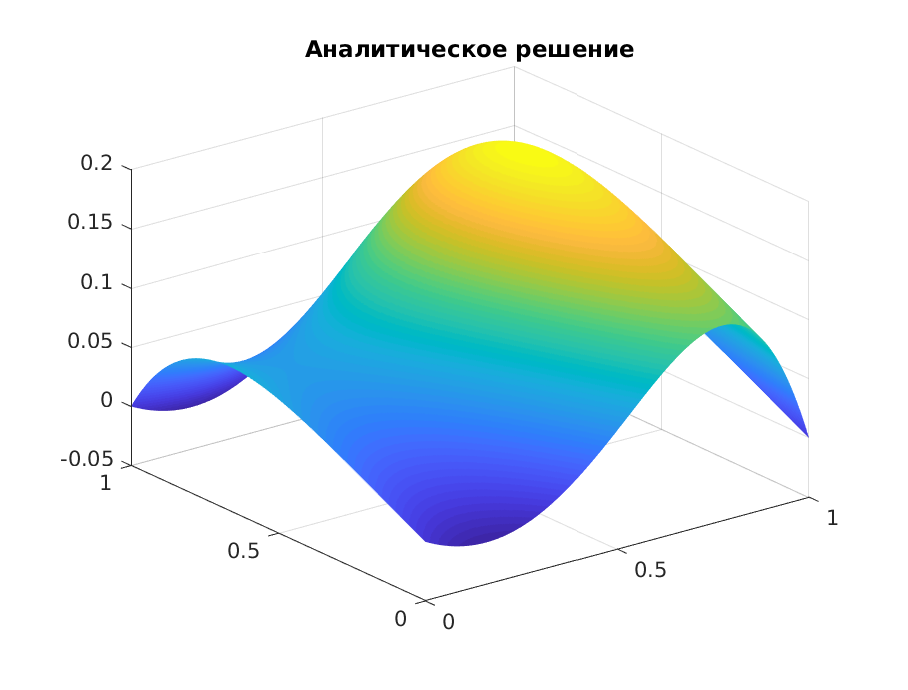
\includegraphics[width=0.51\textwidth]{sol_a_1.eps}
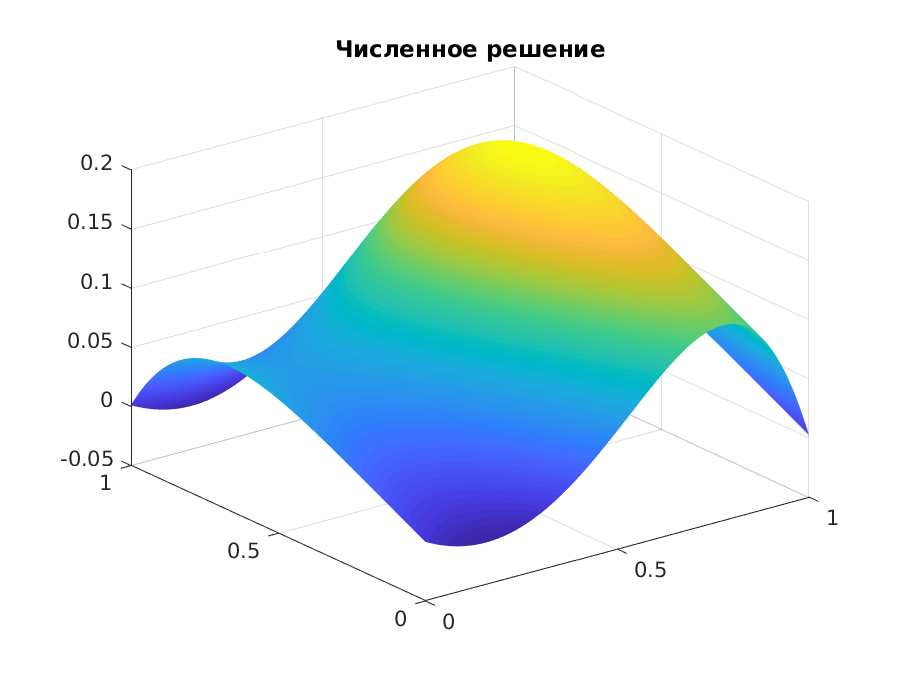
\includegraphics[width=0.51\textwidth]{sol_n_1.eps}
\begin{center}
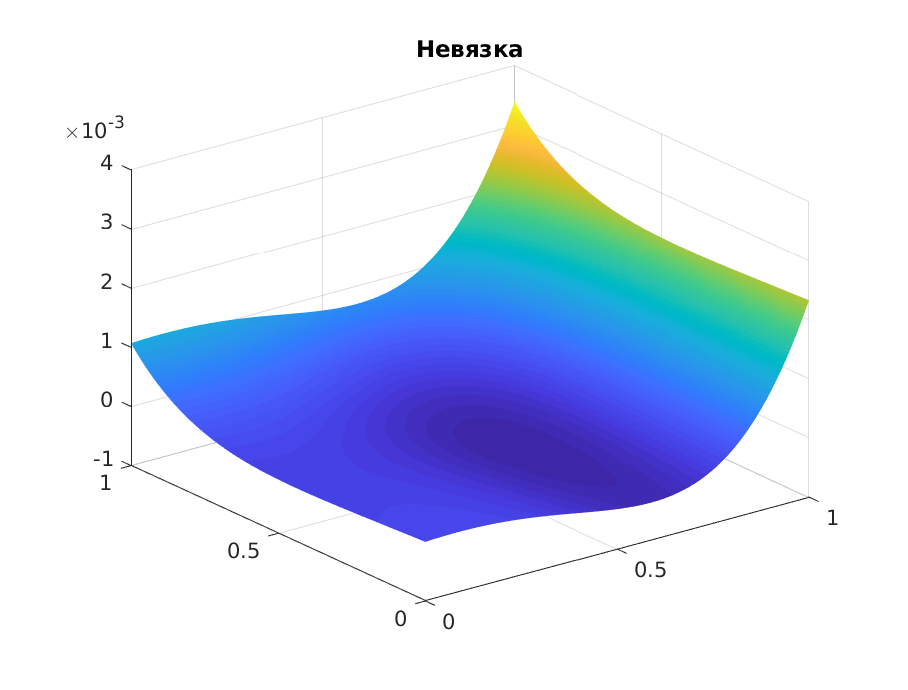
\includegraphics[width=0.7\textwidth]{resid1.eps}

\it{рис. 1 \quad $\mu = 1, \quad u_1^0 = u_2^0 = 0, \quad M = N = 500.$}
\end{center}

\newpage
\noindent
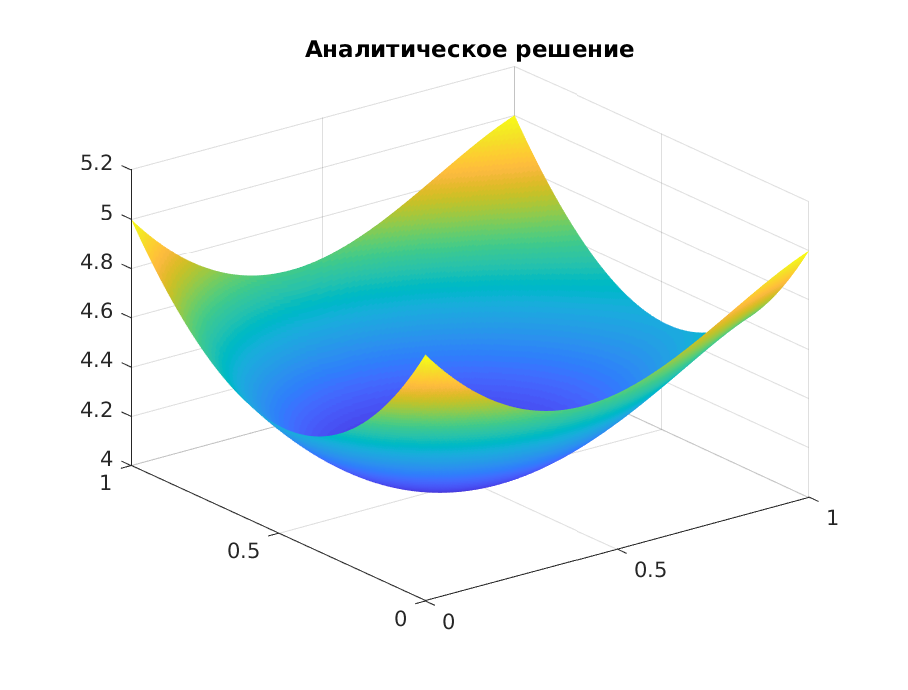
\includegraphics[width=0.51\textwidth]{sol_a_2.eps}
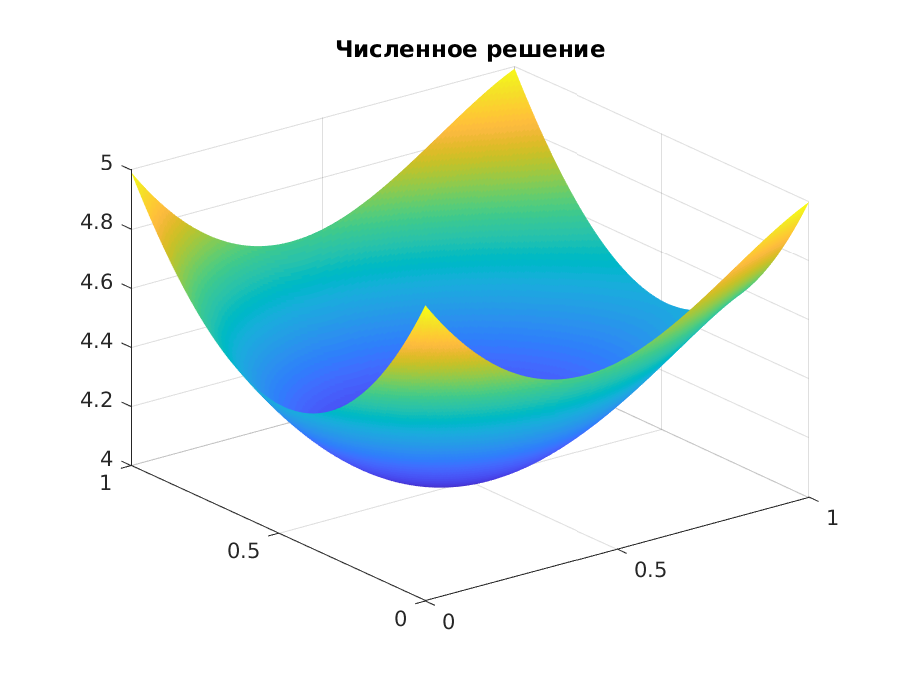
\includegraphics[width=0.51\textwidth]{sol_n_2.eps}
\begin{center}
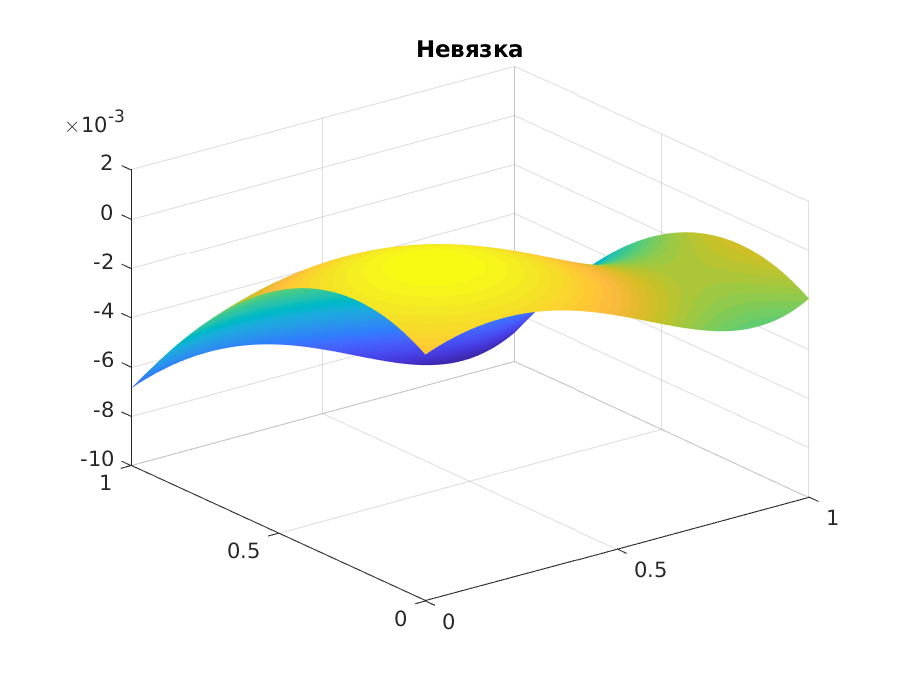
\includegraphics[width=0.7\textwidth]{resid2.eps}

\it{рис. 2 \quad $\mu = 2, \quad u_1^0 = 2, \quad u_2^0 = 3, \quad M = N = 300.$}
\end{center}


\newpage
\noindent
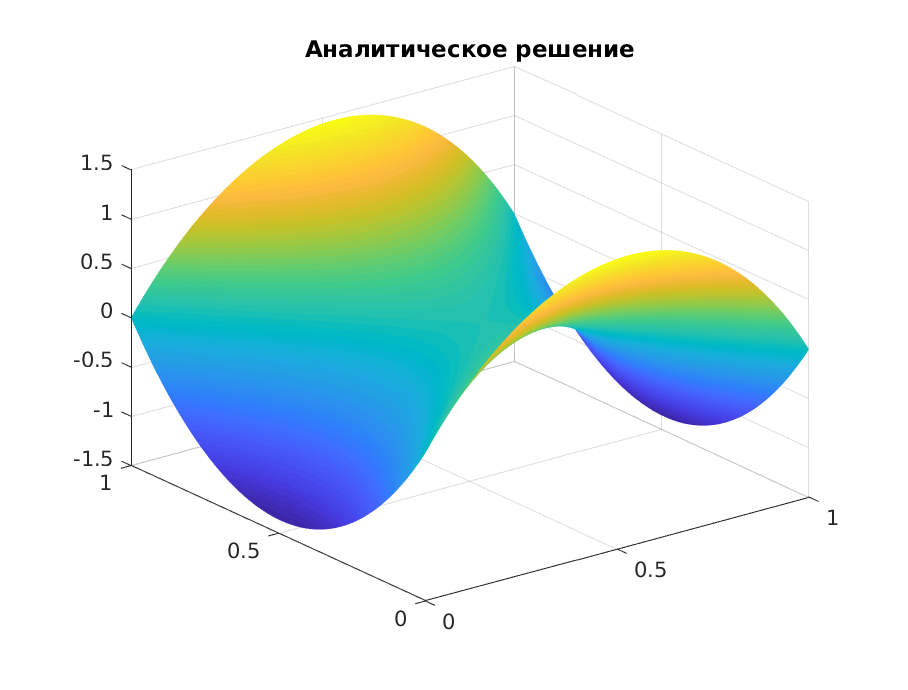
\includegraphics[width=0.51\textwidth]{sol_a_3.eps}
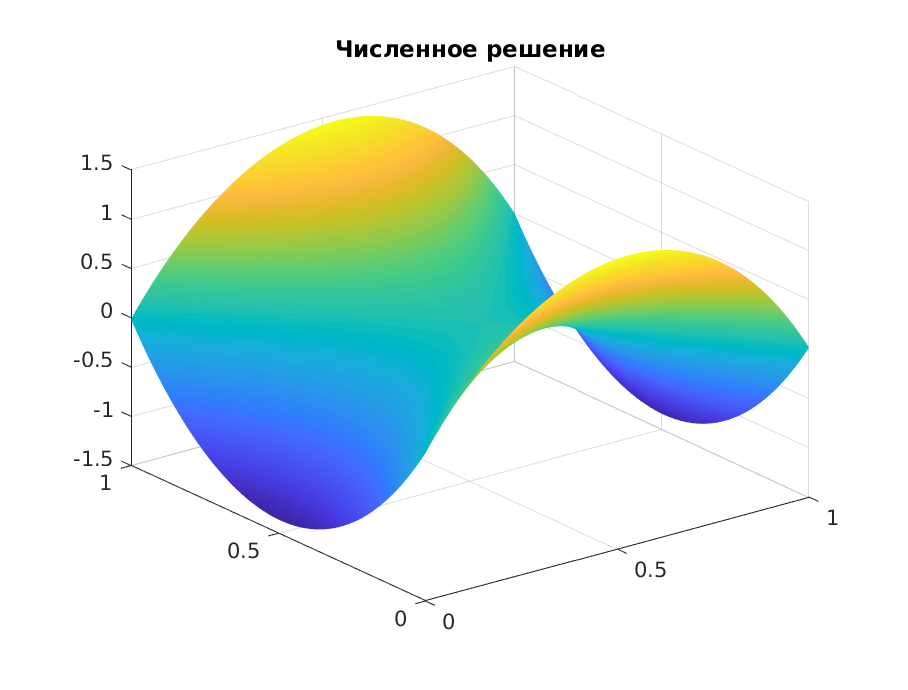
\includegraphics[width=0.51\textwidth]{sol_n_3.eps}
\begin{center}
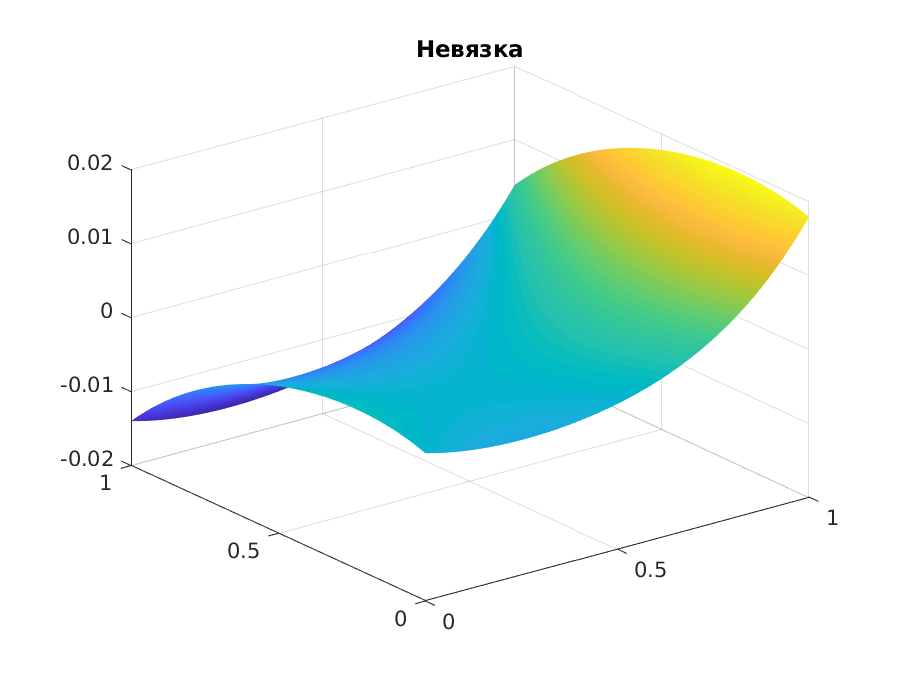
\includegraphics[width=0.7\textwidth]{resid3.eps}

\it{рис. 3 \quad $\mu = 4, \quad u_1^0 = -4, \quad u_2^0 = 4, \quad M = N = 400.$}
\end{center}

В этом примере ошибка численного алгоритма является достаточно большой, однако точность можно повысить измельчением сетки.
\newpage
\noindent
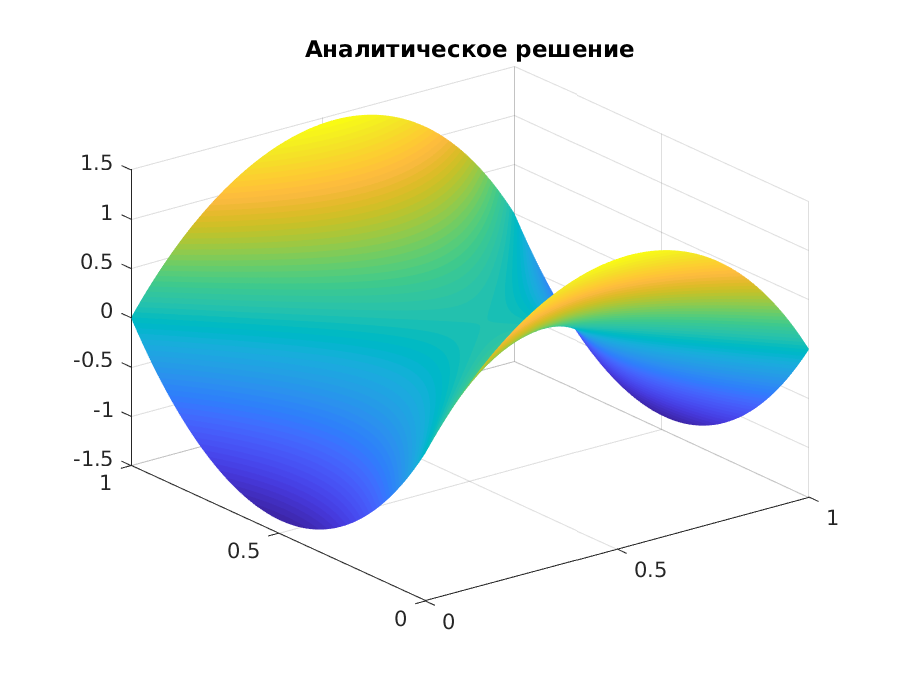
\includegraphics[width=0.51\textwidth]{sol_a_4.eps}
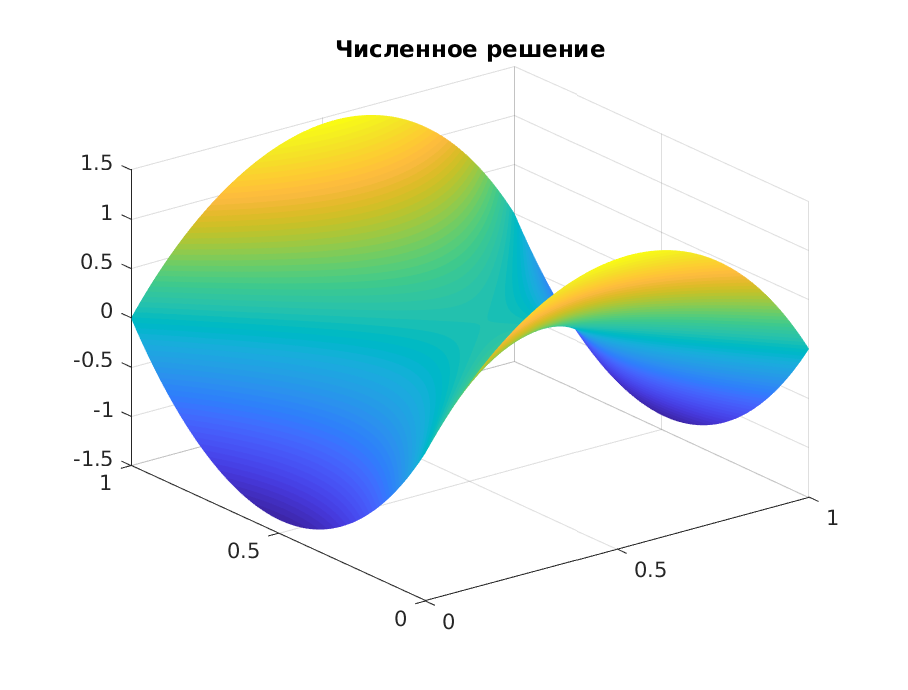
\includegraphics[width=0.51\textwidth]{sol_n_4.eps}
\begin{center}
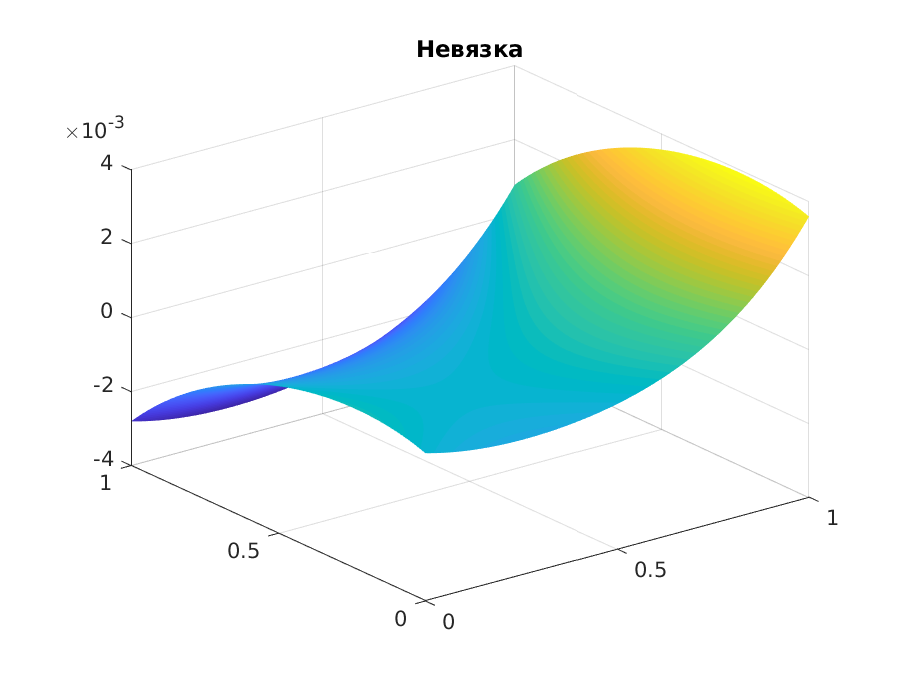
\includegraphics[width=0.7\textwidth]{resid4.eps}

\it{рис. 4 \quad $\mu = 4, \quad u_1^0 = -4, \quad u_2^0 = 4, \quad M = N = 2000.$}
\end{center}

\newpage
\section{Численное решение для произвольной функции}
Пусть $f(x, y) = yx\ln(x) - y^3x^2, \quad \xi(x) = \frac{3}{4}+\left(x-\frac{1}{2}\right)^2, \quad \eta(y) = \sin(\pi y) + 1$. Решения при различных $\mu, M, N$ имеют вид

\noindent
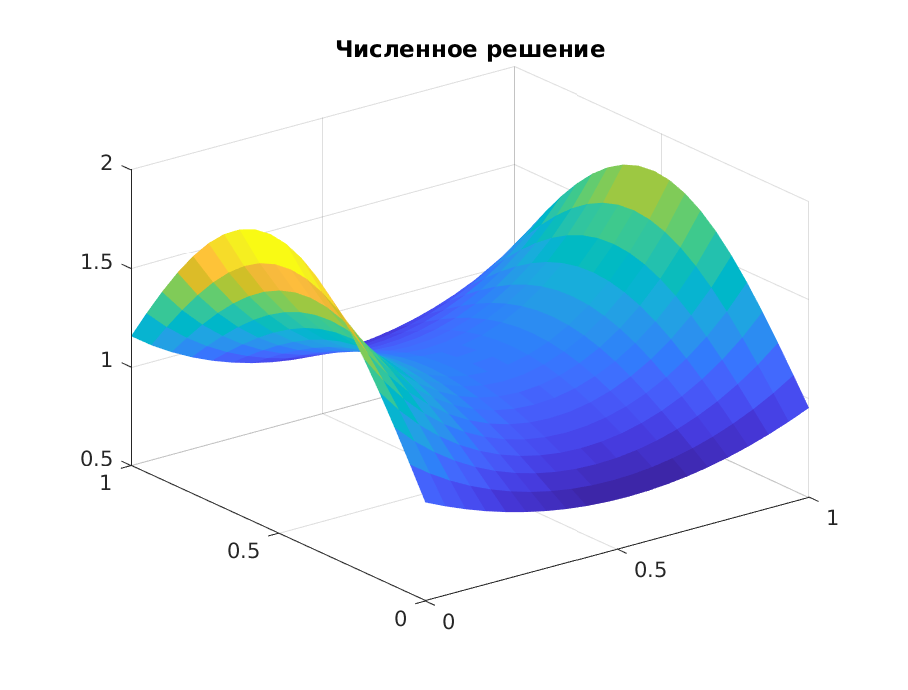
\includegraphics[width=0.51\textwidth]{some1.eps}
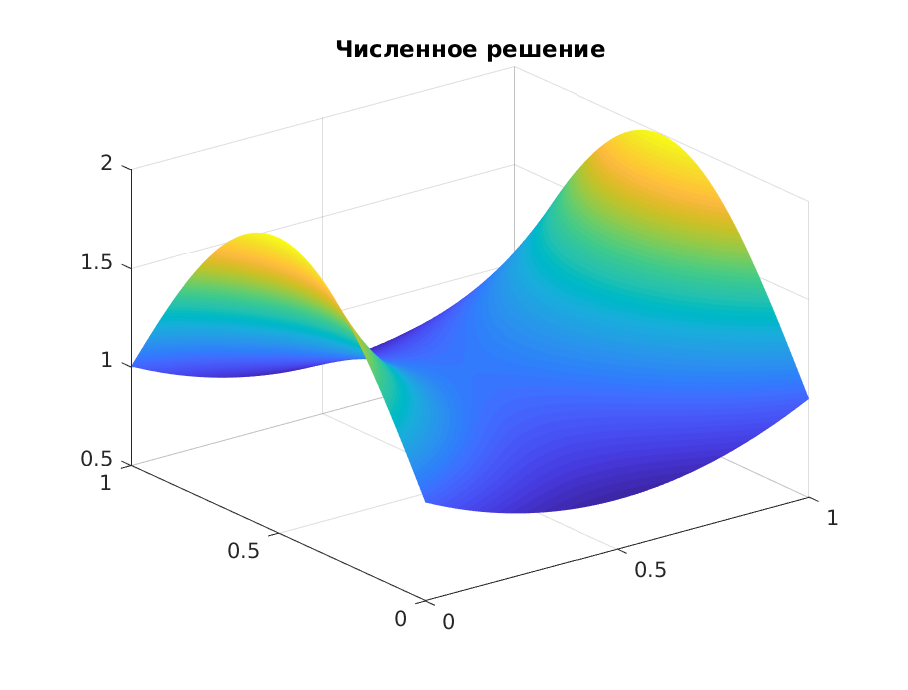
\includegraphics[width=0.51\textwidth]{some2.eps}
\begin{center}
\it{рис. 5 \quad $\mu = 3, \quad M = N = 20.$ \qquad \qquad \qquad \qquad  рис. 6 $\quad \mu = 3, \quad M = N = 1000.$}
\end{center}

\noindent
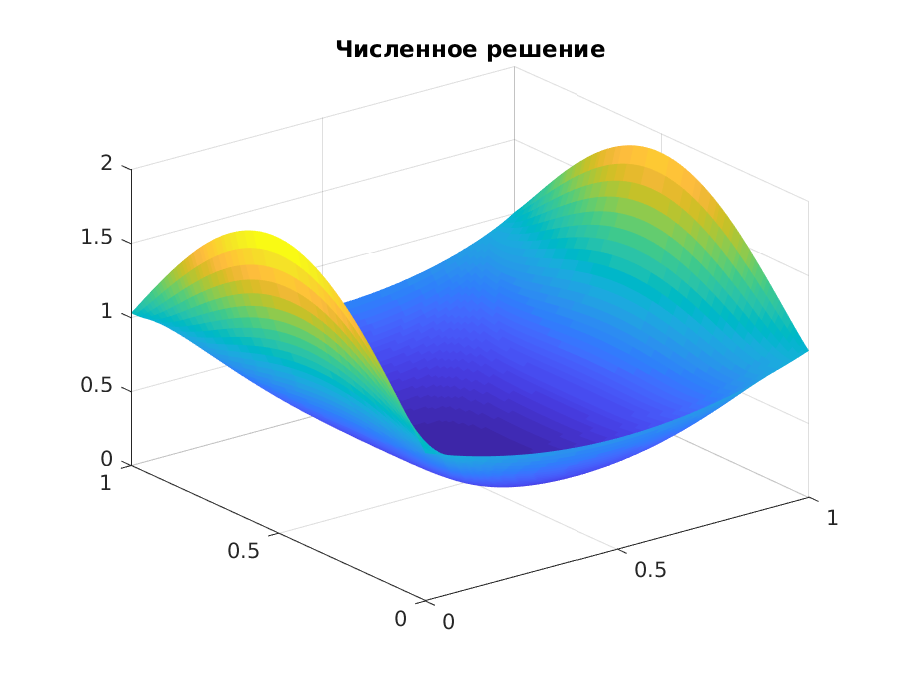
\includegraphics[width=0.51\textwidth]{some3.eps}
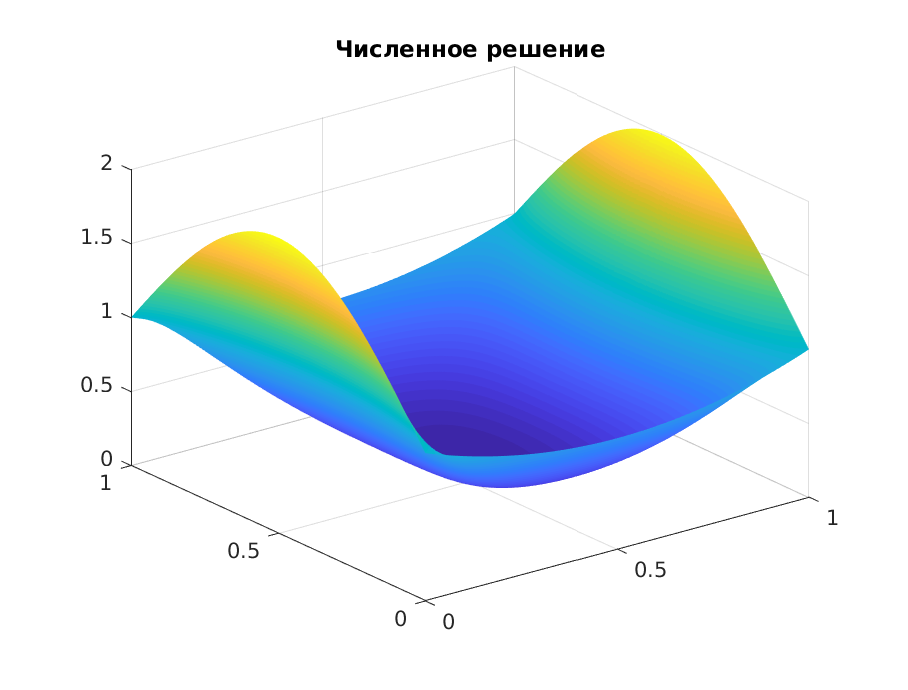
\includegraphics[width=0.51\textwidth]{some4.eps}
\begin{center}
\it{рис. 7 \quad $\mu = 42, \quad M = N = 100.$ \qquad \qquad \qquad \qquad  рис. 8 $\quad \mu = 42, \quad M = N = 1500.$}
\end{center}

\newpage
Рассмотрим теперь $f(x, y) = \cos(xy^2)e^{x-y}, \quad \xi(x) = 0, \quad \eta(y) = 0$. 

\noindent
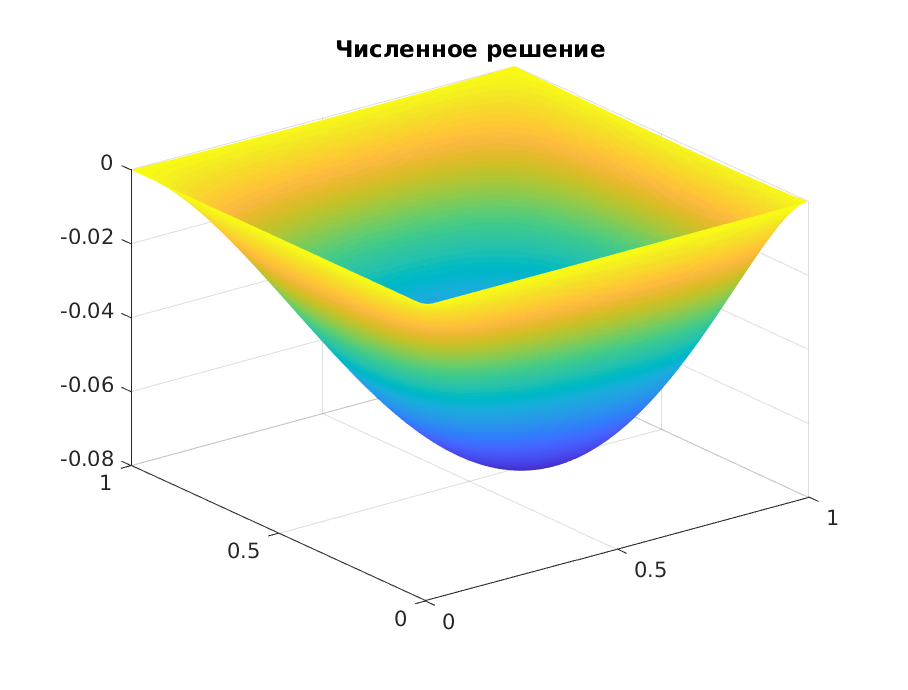
\includegraphics[width=0.51\textwidth]{some5.eps}
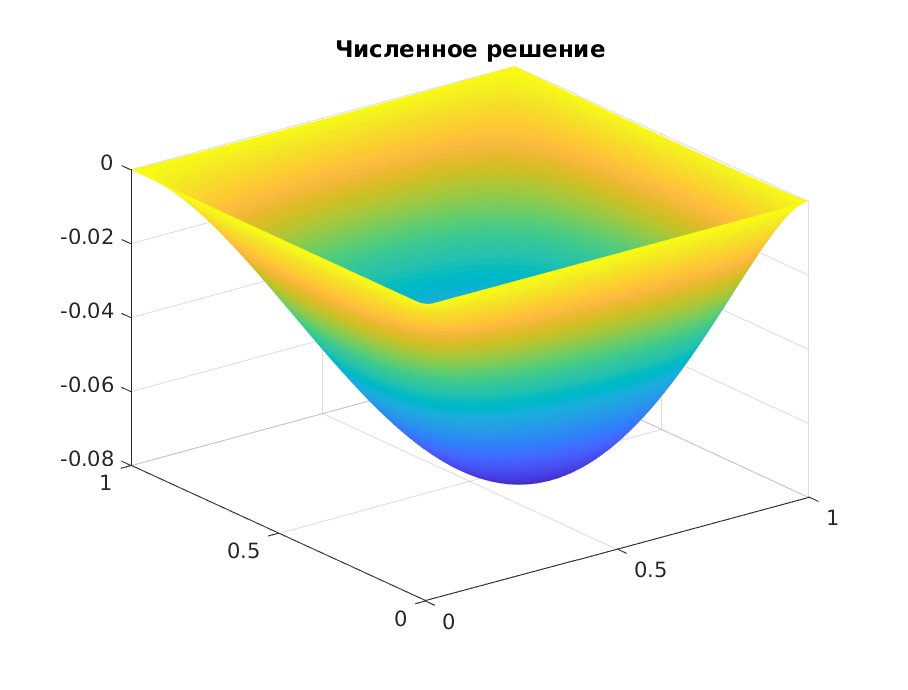
\includegraphics[width=0.51\textwidth]{some6.eps}
\begin{center}
\it{рис. 9 \quad $\mu = 1, \quad M = N = 500.$ \qquad \qquad \qquad \qquad  рис. 10 $\quad \mu = 0.0001, \quad M = N = 700.$}
\end{center}

\noindent
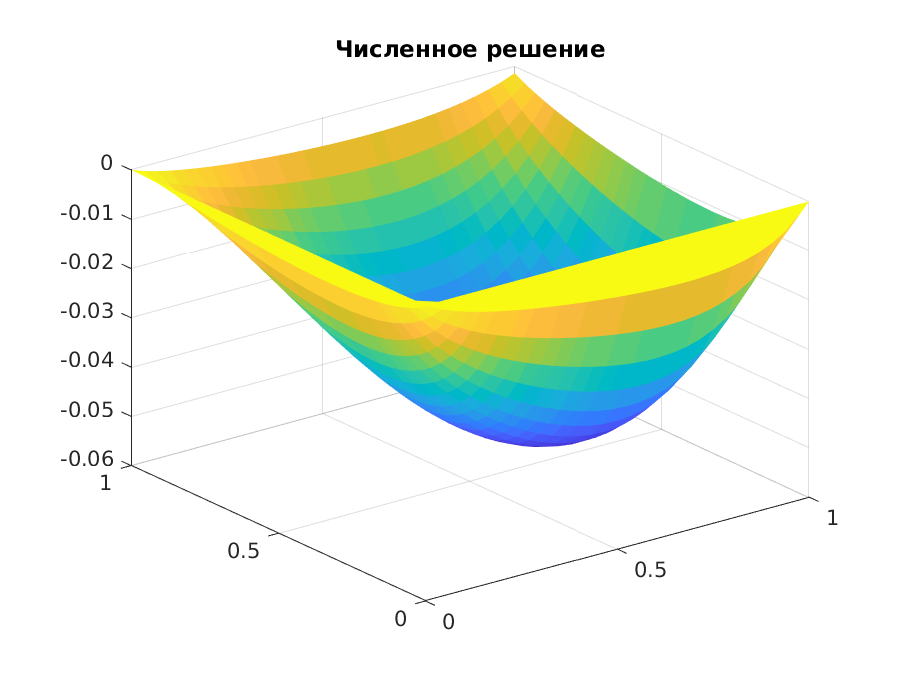
\includegraphics[width=0.51\textwidth]{some7.eps}
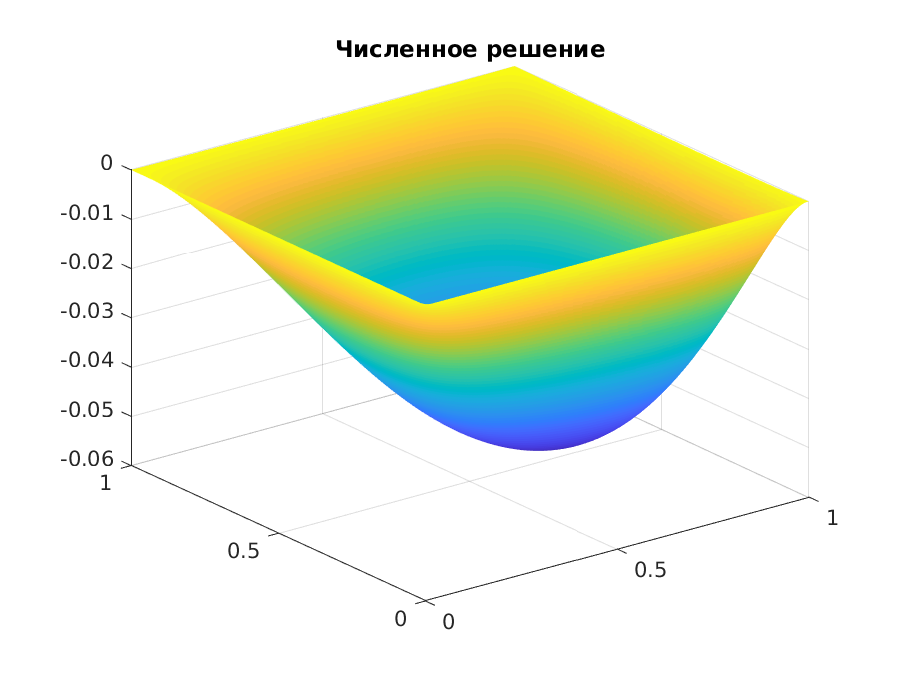
\includegraphics[width=0.51\textwidth]{some8.eps}
\begin{center}
\it{рис. 11 \quad $\mu = 10, \quad M = N = 30.$ \qquad \qquad \qquad \qquad  рис. 12 $\quad \mu = 10, \quad M = N = 1000.$}
\end{center}

\end{document}

